\chapter{Felhasználói dokumentáció} % User guide
\label{ch:user}

Ezen fejezet taglalja a program futtatásához és használatához szükséges információkat. A felhasználói felület is tartalmaz rövid leírást, de a program részletes használati útmutatója a soron következő alfejezetben lesz megtalálható. A programmal egy virtuális teret lehet bejárni, melynek talaján minden irányban végtelen sok mozdíthatatlan gömb található. Van a térben továbbá egy nem aktívan mozgó, de testre szabható fraktálunk, valamint vannak mindenfelé kilőhető és mindenről visszapattanó labdák, melyek a programban megírt fizika alapján viselkednek.


\section{Felhasználói felület és funkciók} 
\label{sec:ui} 
A program sikeres indítása után -- melyről \aref{sec:futtatas}. fejezetben tudhatunk meg többet -- kettő darab ablakkal találjuk szembe magunkat. Ezekről \aref{fig:Kezdokepernyo}. és \ref{fig:Terminal}.~ábrák mutatnak egy-egy képernyőképet.

\Aref{fig:Kezdokepernyo}. ábrán látható ablak tartalmazza a program lényeges részét, itt jelenik meg a kirajzolt képünk és ebben az ablakban található a \textbf{``Parameters''} feliratú panel, melynek segítségével különböző paramétereket tudunk nyomon követni és módosítani. Az ablak alapértelmezetten 1920x1080 nagyságú, de szabadon átméretezhető, viszont az ablak mérete befolyással van a teljesítményre! Mindig az ablak pontos felbontásában fog renderelni, így nem optimális teljesítmény esetén érdemes megfontolni az ablak kisebbre vételét.

\begin{figure}[H]
	\centering
	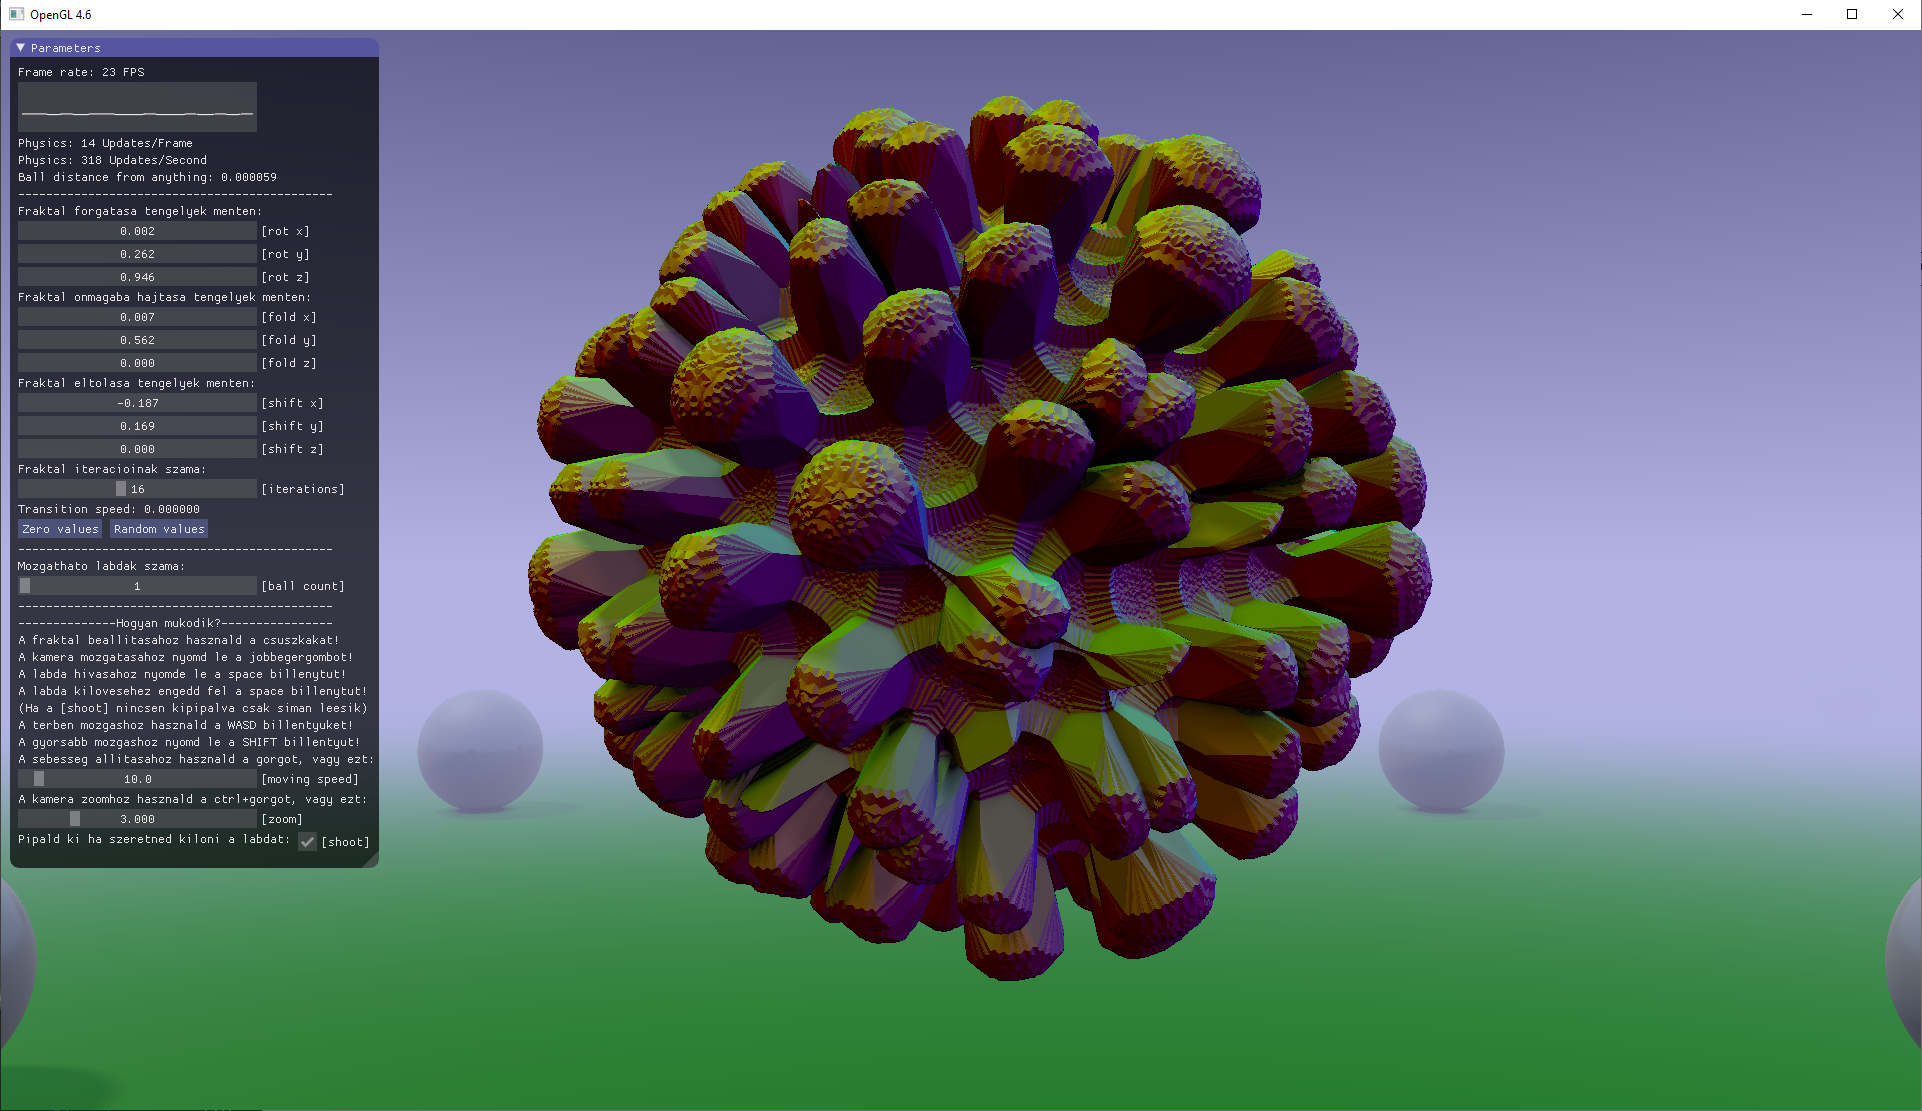
\includegraphics[width=0.9\textwidth,frame]{Kezdokepernyo}
	\caption{Fő programablak}
	\label{fig:Kezdokepernyo}
\end{figure}

\Aref{fig:Terminal}. ábrán vehetjük szemügyre azt a terminálablakot mely az esetleges hibaüzeneteket fogja kiírni. Ezen kívül ez az ablak más funkcióval nem bír.

\begin{figure}[H]
	\centering
	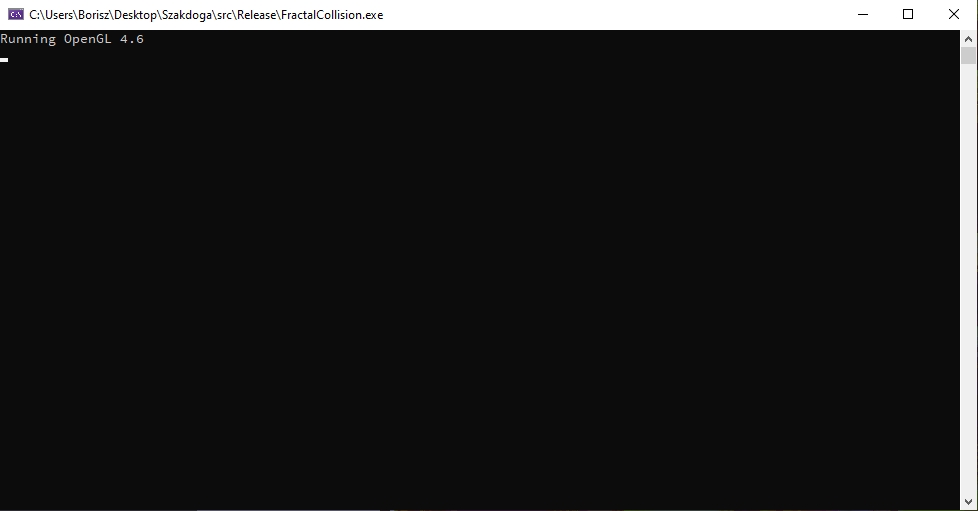
\includegraphics[width=0.9\textwidth,frame]{Terminal}
	\caption{Terminálablak}
	\label{fig:Terminal}
\end{figure}

\subsection{A ``Parameters'' feliratú panel}

A \textbf{``Parameters''} feliratú panel nagy jelentőséggel bír, így a jobb olvashatóság végett nem csak \aref{fig:Kezdokepernyo}~ábra részeként láthatjuk hanem külön is szerepel \aref{fig:Parameters1}., \ref{fig:Parameters2}. és \ref{fig:Parameters3}.~ábrákon.

Ezen a panelen számos információt tudhatunk meg és állíthatunk át a program futásával kapcsolatosan. Alapértelmezetten a fő programablak bal oldalán található, de szabadon mozgatható és átméretezhető az ablakon belül, indításkor pedig az legutóbbi futtatás végén beállított pozíciót és méretet veszi fel. 

\begin{figure}[H]
	\centering
	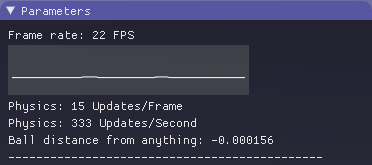
\includegraphics[width=0.4\textwidth,frame]{Parameters1}
	\caption{A ``Parameters'' feliratú panel felső harmada}
	\label{fig:Parameters1}
\end{figure}

A panel legtetején (\ref{fig:Parameters1}.~ábra) találhatjuk a \textbf{``Frame rate:''} felirat után az aktuális képfrissítési rátát képkocka/másodperc mértékegységben, illetve közvetlenül ezalatt az utolsó másfél másodperc adatait követhetjük nyomon egy folyamatosan frissülő grafikonon. 

A két \textbf{``Physics:''} felirat után olvashatjuk le hogy milyen gyakran van a labdák mozgása frissítve frissítés/képkocka és frissítés/másodperc mértékegységekben. Egy frissítés során minden labda sebessége és pozíciója újraszámolódik, valamint ellenőrzésre kerül az is hogy ütközött-e valamivel. 

A \textbf{``Ball distance from anything:''} felirat után olvasható a dobálható labda távolsága a tőle legközelebb lévő felülettől - több labda esetén az utoljára létrehozottra vonatkozik. Az apró ingadozásából látszik hogy igazából folyamatosan pattog a labda, csak ez a pattogás egy idő után elhanyagolható mértékű lesz.

\begin{figure}[H]
	\centering
	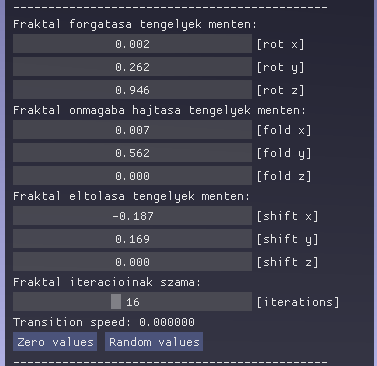
\includegraphics[width=0.4\textwidth,frame]{Parameters2}
	\caption{A "Parameters" feliratú panel középső harmada}
	\label{fig:Parameters2}
\end{figure}

A választóvonal alatti szekcióban (\ref{fig:Parameters2}.~ábra) a fraktálunkat tudjuk személyre szabni. A fraktálunk úgy rajzolódik ki hogy egy 1x1x2 egység nagyságú téglatesten egymás után többször végrehajtunk különböző transzformációkat. Ezen transzformációk paramétereit tudjuk beállítani a következő 9 db határ nélküli csúszkán - mely ugyanúgy működik mint egy sima csúszka, csak nincsen minimum és és maximum értéke és az egeret tovább is lehet húzni mint a csúszka vége. Mindegyik csúszkának CTRL + kattintással begépelt értéket is meg lehet adni. 

A \textbf{[rot x], [rot y], [rot z]} csúszkákkal azt tudjuk szabályozni hogy mennyire legyen elforgatva egy iterációban a fraktál az X, Y és Z tengelyek körül (radiánban értendők az értékek). 

A \textbf{[fold x], [fold y], [fold z]} csúszkákkal azt tudjuk szabályozni hogy mennyire legyen elforgatva az adott tengely körül a tükrözősík  ami a megadott szöggel (radián) fordul el és tükrözi az alakzatot iterációnkként. Itt a három érték 3 különböző tükrözősíkot forgat el a nevükben szereplő tengely mentén. 

A \textbf{[shift x], [shift y], [shift z]} csúszkák szabályozzák hogy mennyire legyen eltolva az alakzat iterációnként az X, Y és Z tengely mentén.

Végül pedig az \textbf{[iterations]} csúszka, amely már korlátozva van az [1,36] tartományban, beállítja hogy az előző 9 csúszka által paraméterezett 9 transzformáció hányszor legyen végrehajtva a téglatesten. Ez a paraméter van a legnagyobb hatással a futás sebességére, így gyengébb gépeken nem érdemes nagy értéket beállítani. Ha a képfrissítési ráta 10 képkocka/másodperc alá csökken akkor automatikusan elkezd csökkenni a csúszka értéke.

Itt található még két gomb: a \textbf{``Zero values''}, mely a fraktál paramétereket nullához közelíti\footnote{Az értékek csak konvergálnak a 0-hoz. Ha valamely paraméter szélsőségesen nagy, előfordulhat hogy a gomb megnyomása után is jelentősen eltér nullától}, illetve a \textbf{``Random values''}, mely véletlenszerű értékeket állít be ezeknek. Az iterációk számát egyik sem állítja át. Továbbá van még egy ezekhez szorosan kacsolódó érték ami a \textbf{´´Transition speed:''} felirat után olvasható. A gombok által generált új paramétereket egy 5 másodperc hosszú fázisban folyamatosan, apránként közelíti az aktuális paraméterekkel, az előbb említett érték pedig azt fejezi ki hogy milyen súlyozással veszi az aktuális és a célérték átlagát.

\begin{figure}[H]
	\centering
	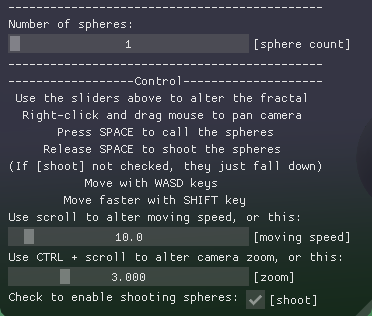
\includegraphics[width=0.4\textwidth,frame]{Parameters3}
	\caption{A "Parameters" feliratú panel alsó harmada}
	\label{fig:Parameters3}
\end{figure}

Az alsó harmadban (\ref{fig:Parameters3}.~ábra) található a \textbf{[sphere count]} csúszka, itt 1 és 100 között lehet értékeket beállítani. Ez is jelentősen befolyásolja a futás gyorsaságát, így 15 FPS alatt ez az érték is automatikusan csökken.

Van egy rövid ismertető szövege a panelnek, ami azt a célt szolgálja hogy ezen dokumentáció nélkül is tudja használni egy felhasználó ha leül a program elé. Ebben kerülnek ismertetésre a virtuális tér bejárásához szükséges irányítások is. A mozgáshoz a \textbf{WASD} billentyűket és az egeret lenyomott jobb egérgombbal\footnote{Erre azért volt szükség mert a paraméterek beállításához is az egeret kell használni, muszáj volt elkülöníteni valahogy a kettőt} kell használni a legtöbb játékban megszokott módon -- a kamera szabadon repül bármilyen irányba. A mozgási sebességet a \textbf{[moving speed]} csúszkával lehet személyre szabni, illetve ugyanezen csúszka értékét az \textbf{egérgörgővel} is lehet szabályozni. A \textbf{shift} billentyű lenyomására ideiglenesen megnégyszereződik a sebesség, felengedésére visszaáll. A kamera látószögét lehet csökkenteni a \textbf{[zoom]} csúszka értékének növelésével, vagy a \textbf{CTRL + görgő} segítségével is.

A labdákat a \textbf{szóköz} billentyű nyomva tartásával lehet magunkhoz hívni. Egy labda esetén az ablak közepére, több labda esetén a labdák az ablak közepe körül keringenek egy körvonal mentén egyenletesen elhelyezkedve. A szóköz billentyűt felengedve egyszerre kilövődnek a labdák, ha be van pipálva a panel alján a \textbf{[shoot]} jelölőnégyzet, ha nincsen bepipálva csak leesnek a gravitációnak megfelelően.
 
\cleardoublepage
\section{Rendszerkövetelmények és futtatás} 
\label{sec:futtatas} 
Az alkalmazás üzembe helyezésének egyetlen követelménye a Windows 7 vagy afeletti operációs rendszer. Azonban az alkalmazás rettentően GPU intenzív, így az optimális futáshoz elengedhetetlen a dedikált videokártya. A teszteléshez használt számítógép specifikációi:
\begin{compactitem}
	\item Intel® Core™ i7-8700 CPU
	\item 16 GB RAM
	\item NVIDIA GeForce GTX 1660 GPU
	\item Windows 10 operációs rendszer
\end{compactitem}
Ezen konfigurációval, 1920x1080 felbontás mellett a program sebessége elfogadható volt.

Az alkalmazás elindításához a \textbf{FractalCollision.exe} fájlt kell futtatni. Fontos hogy az exe fájl mellett ott legyen a \textbf{shader.frag} és a \textbf{shader.vert} fájlok, illetve ha a rendszeren nincsen külön telepítve akkor az \textbf{SDL2.dll}, valamint a \textbf{glew32.dll} fájloknak is az exe mellett kell lenniük. Ezek mind a \textbf{Release} mappában vannak, így onnan indítva erre nem kell ügyelni.

Az alkalmazásból való kilépéshez lehet az \textbf{ESC} billentyűt vagy a jobb felső sarokban az ablak bezárás gombját használni. Ha bezárjuk a terminálablakot akkor mindkét ablak bezárul, ha először a fő programablakot zárjuk be akkor utána még külön be kell zárni a terminálablakot.

Az alkalmazás \textbf{Microsoft Visual Studio} segítségével készült, így ha újra akarnánk fordítani akkor a \textbf{C:/} helyre csomagoljuk ki a mellékelt OGLPack.zip állományt (ez az OpenGL-hez szükséges fájlokat tartalmazza), majd futtassuk a \textbf{subst T: C:/} parancsot. Ezután megnyithatjuk a \textbf{.vcxproj} projektfájlt.


